\documentclass{article}

\usepackage{amsmath}
\usepackage{amscd}
\usepackage[tableposition=top]{caption}
\usepackage{ifthen}
\usepackage[utf8]{inputenc}
\usepackage{longtable,pdflscape} 
\usepackage{mathptmx}
\usepackage{hyperref}
\usepackage{Sweave}
\usepackage{tikz}
\usepackage{pgf}
\usepackage{a4wide}


% \VignetteIndexEntry{IPMpack: An R Package for demographic modeling}
% \VignetteDepends{Matrix, MASS, nlme, mvtnorm, methods}
% \VignetteKeyword{kwd1}
% \VignetteKeyword{kwd2}

%\SweaveOpts{prefix.string=Guide/} 
 
\begin{document}

\title{IPMpack: an R package for demographic modeling with Integral Projection
Models (v.1.5)}
\author{Jessica Metcalf, Sean M. McMahon, Rob Salguero-Gomez, Eelke Jongejans}
\maketitle


%\section*{IPMpack: an R package for demographic modeling}
%\makeabstract
The goal of IPMpack is to provide a suite of demographic tools based
on Integral Projection Models (IPMs) to support biologists interested in
making projections for populations where demography is strongly linked to a changing continuous variable, such as size. The package includes functions that can take data, such as size or age, as well as environmental covariates, and build models of growth, survival and fecundity. Functions are defined that then take these
statistical models and construct IPMs. IPMpack has tools that compare different
functional forms for the underlying statistical models, plotting them and
returning model scores, as well as tools for diagnostic tests of the IPM models
themselves. There are also methods to build population models for varying environments, use Bayesian methods to sample population parameters,  estimate longevity and passage time, sensitivity and elasticity (of either parameters or matrix elements), and much more.

This vignette is intended to introduce the concepts of IPMs as well as the
implementation of IPMpack to biologists with a wide range of quantitative skills.  This vignette is for IPMpack version $1.5$, and so we encourage users to contact the IPMpack team at \href{IPMpack@gmail.com}{IPMpack@gmail.com} with any feedback or mistakes they find.  We also host a blog at R-forge (http://ipmpack.r-forge.r-project.org/) that contains news of updates, new features, and announcements of papers and meetings relevant to IPMs.
 
\newpage

\section{Introduction to Integral Projection Models}
An Integral Projection Model (IPM) is a demographic tool that can estimate the
dynamics of populations where individuals' fates depend on state variables that
are continuous (e.g., weight, diameter at breast height, height, limb length,
rosette diameter) or quasi-continuous (e.g., number of leaves, age, number of
reproductive structures) and may be a mixture of discrete and continuous
variables. IPMs track the distribution of individuals $n$ across these state
variables between census times (e.g., year $t$ and year $t+1$) by projecting from models that define the underlying vital rates (e.g., survival, growth, and reproduction) as a function of the (quasi-)continuous state variables. For detailed introductions to IPMs see Easterling et al. ($2000$), and Ellner \& Rees ($2006$, $2007$).

Briefly, an IPM is defined by a kernel $K$ that represents probabilities of growth between discrete or continuous stages, survival across these stages, and the production of offspring and offspring recruitment.  For example, in the simplest case, where the population is structured by a continuous covariate, size, then 
\begin{equation}
n(y, t+1) = \int\limits_{L}^{U} K(y, x) n(x, t) \, dx       
\end{equation}
where $n(y, t+1)$ is the distribution across size $y$ of both established and new individuals in census time $t+1$, $n(x, t)$ the distribution across size of individuals in census time $t$, and $L$ and $U$ the lower and upper size limits modeled in the IPM, respectively. 

Multiple functional forms for both demographic processes as well as their error
structures can be  accommodated with IPMpack. The $F$ kernel (equation 4)
describes per-capita contributions of reproductive individuals to number of new
individuals at the next census. Multiple size-dependent or size-independent
vital rates can be fitted within the $F$ kernel, reflecting for example
reproductive probability, number of reproductive structures (e.g. flowers in
plants, basidia in fungi), number of propagules within reproductive structure
(e.g. seeds in inflorescences), and so on. Additionally, a range of constants
($c_1$, $c_2$, ...) can be included if there are no data for a stage. All of these will be multiplied to obtain the eventual fertility for individuals of each size. Finally, the $F$ kernel definition includes a probability density function describing the size of offspring recruiting into the population, $f_d$. 

From equation 1: 
\begin{equation}
n(y, t+1) = \int\limits_{L}^{U} K(y, x) n(x, t) dx = \int\limits_{L}^{U}
[P(y, ) + F(y, x)] n(x, t) dx ,
\end{equation}

where

\begin{equation}
 \int\limits_{L}^{U} P(y, x) n(x, t) dx = \int\limits_{L}^{U}surv(x)growth(y, x)dx ,    
\end{equation}
and
\begin{equation}
 \int\limits_{L}^{U} F(y, x) n(x, t) dx = \int\limits_{L}^{U}
c_1 c_2 c_3 ... fec1(x)fec2(x)fec3(x)...f_d(y, x)dx     
\end{equation}
After numerically solving these kernels, key ecological and evolutionary quantities such as the population rate of increase $\lambda$, the stable population size structure, the net reproductive rate $R_0$, and many others can be estimated (see Caswell $2001$ for more a comprehensive discussion). 

Essentially, the same tools are available for IPMs as for discrete projection
matrices (matrix population models), e.g., estimation of population
growth rate, sensitivities, elasticities, life table response
experiment [LTRE] analyses, passage time calculations, etc. (Caswell
$2001$, Cochran \& Ellner $1992$, and others); as well as some
additional tools based on exploring the impact of the underlying
statistical relationships. The main difference
between an IPM and a matrix model is that while in discrete projection
matrices the number of classes (i.e., number of stages in the life
cycle of the study species) must be defined {\tt a priori}, IPMs
impose the discretization of the three-dimensional surface defined by
equation 1 in the last step for the purposes of numerical integration. This produces a typically large matrix (e.g., $100$ x $100$ cells) that is more robust to biases from matrix dimensionality (Zuidema et al. $2010$, Salguero-Gomez \& Plotkin $2010$) and sample size (Ramula et al. $2009$) than classical matrix models.

The goal of IPMpack is to provide a centralized set of quantitative techniques based on IPMs to help ecologists and evolutionary biologists model populations. IPMpack can accommodate multiple vital rates from complex life cycles all grouped into two main sub-kernels: $P$ and $F$ (equation 2) \footnote{Note than in the seminal paper by Easterling et al. ($2000$) this kernel was referred to as $P$, but here we follow the terminology by Caswell ($2001$) and call it $P$ instead). The $P$ kernel (equation 3) describes {\tt growth} between demographic censuses conditional on individuals' survival ({\tt surv}).
}.

This vignette walks through the steps of a basic IPM analysis.  We first
describe the kind of data necessary to build an IPM.  If a user begins `from
scratch', they must input data in a specific format (described below).  However
it is possible to jump past this step and use IPMpack capabilities on IPMs that
were developed outside of IPMpack. That is, if a user wants quick figures, summary statistics, other analyses on an IPM matrix already built, IPMpack can readily accommodate that.   However there are some features that, because of the object-oriented coding, require some specific structures (and other features that do not).  Please refer to the manual files, and the rest of this vignette for this information. The vignette will begin with data input.  We will then walk through how to build and analyse a basic IPM model.  More complex models will be introduced later, as well as run comparative model testing and Bayesian implementations.

\section{Getting started: setting up the data for IPMpack}
For users who prefer to define IPM matrices using their own
statistical tools, there is no requirement for the data to be in any
particular format, and most of the functions in IPMpack will operate
on the matrices directly (e.g., life expectancy, sensitivity of matrix
elements, etc.).  However, to use IPMpack's full capacities, the
individual-level demographic data must be organized in a {\tt data frame} (a
class of object in R [see help file for `data.frame' in base]), where each row
represents one observation of an organism in the population at one census time
$t$ with the following potential column names:
\begin{itemize}
\item  {\tt size}: size of individuals in census time $t$  $^*$
\item  {\tt sizeNext}: size of individuals in census time $t+1$  $^*$
\item  {\tt surv}: survival of individuals from census time $t$ to  $t+1$ (contains: 0 for death or 1 for survival) $^*$
\item  {\tt fec1, ...}: as many columns as desired relating size to sexual reproduction. For example, this might be: 
  \begin{itemize}
  \item {\tt fec1}: probability of reproduction (output: 0 for no reproductive or 1 for reproductive)
  \item {\tt fec2}: number of reproductive structures (output: 1, 2, 3, $...$) when individual is reproductive, that is, when fec1 = 1
  \item {\tt fec3}: number of propagules (output: 1, 2, 3, $...$) per reproductive structure (e.g. seeds per flower in reproductive plant individual)
  \item ...
  \end{itemize}
\item  {\tt stage}: stage of individuals in census time $t$, used to
  distinguish discrete and continuous stages, etc. For rows in the  data frame where {\tt size} is not an NA, then this must be the word ``continuous''. Where {\tt size} is NA, any variety of named discrete stages  may be defined (e.g. ``seed bank''). If this column is missing, many procedures in IPMpack are designed to simply fill in this column assuming that only ``continuous'' state variables describe the life cycle of the species, i.e. there are no discrete stages. For running {\tt makeFecObj}, the column must be a factor. If not supplied, the function will generate this column assuming all individuals are "continuous".
\item  {\tt stageNext}: stage of individuals in census time $t+1$, in the
simples case, ``continuous'' or ``dead''(which is redundant with ``0''
in the {\tt surv} column. As above, this column is not essential
for many procedures in  IPMpack. For running {\tt makeFecObj}, the column must be a factor. If not supplied, the function will generate this column assuming all individuals that are alive are ``continuous".
\item  {\tt number}: number of individuals corresponding to each row in the data frame. For all rows corresponding to movement between continuous stages, this value will be $1$, but for movement between  discrete stages (e.g., from ``dormant seeds'' to ``seeds ready to  germinate'') then this number may be $>1$, potentially directly  reflecting observed individuals in the data. This information avoids having a data frame with a row for every discrete stage (e.g. seed). As above, many  procedures in IPMpack will simply assume that this value is always 1. 
\item  {\tt covariate}: value of a discrete covariate in census time  $t$, such as light environment at time $t$, age at $t$, patch at $t$, etc. 
\item  {\tt covariateNext}: value of a discrete covariate in census time $t+1$.
\item  ...any other covariates of interest, named as desired by the user are possible too (e.g., precipitation, habitat, temperature, etc).
\item {\tt offspringNext}: if the size contained in sizeNext corresponds to the
size of an offspring, this column will contain either the value ``sexual" or
``clonal" (depending on whether sexual or clonal reproduction is being
considered). If this column exists, rows that take these two values will be excluded from the growth analyses (functions {\tt makeGrowthObj} and variants thereof, see below).
\end{itemize}

The $^*$ symbol above indicates the minimum columns in the data frame required to obtain passage time and life expectancy calculations. These values form the $P$ kernel. If sufficient additional columns are available, a full life-cycle model, containing the $F$ kernel, can be produced and further analyses are possible.  Although {\tt size} and {\tt sizeNext} can be transformed, many of the utility functions assume no transformations in columns in the original data frame pertaining to fertility. Transformations can be formally called in various parts of the package and appropriate $F$ matrices built that account for these transformations. 

\section{The basics: building an IPM}

First, the user must install IPMpack from CRAN using
{\tt install.packages("IPMpack")} and then load IPMpack into an R session
({\tt library(IPMpack)}) (see help files for problems with installation or loading). 

\begin{Schunk}
\begin{Sinput}
> library("IPMpack")
\end{Sinput}
\end{Schunk}
Next, the user must input demographic data. As mentioned above, most functions of IPMpack require a data file with at minimum columns called {\tt size}, {\tt sizeNext}, {\tt surv}, where `size' is size at time t, `sizeNext' is size one census later, and `surv' is a series of 0s and 1s, indicating if the individual survived or not. In the case of `size' and `sizeNext', data can be transformed (e.g., onto a log scale), if appropriate via functions built into IPMpack. For the purpose of learning how to use IPMpack, the user can either use his/her own data (adjusted to have the appropriate headings, as aforementioned), or generate them with a function built into IPMpack:

\begin{Schunk}
\begin{Sinput}
> dff <- generateData()
\end{Sinput}
\end{Schunk}
A quick check indicates that this contains sensible (fictional) information: 
\begin{Schunk}
\begin{Sinput}
> head(dff)
\end{Sinput}
\begin{Soutput}
      size  sizeNext surv covariate covariateNext        fec      stage
1 5.096741  4.261369    0         1             0 11.7951986 continuous
2 5.453092  4.352565    0         0             0  7.1677199 continuous
3 3.651964  1.053892    0         1             0  1.4883059 continuous
4       NA -1.985458   NA         1             0         NA       <NA>
5 4.431822  3.018367    1         1             0  0.4929436 continuous
6 3.680777  3.358329    0         1             0 14.4894098 continuous
   stageNext
1 continuous
2 continuous
3 continuous
4 continuous
5 continuous
6 continuous
\end{Soutput}
\end{Schunk}

for simplicity, no discrete covariates are included in this first example. Figure~\ref{fig:zero} (p.~\pageref{fig:zero}) is produced by the following code:

\begin{Schunk}
\begin{Sinput}
> plot(dff$size, dff$sizeNext, xlab = "Size at t", ylab = "Size at t+1")
\end{Sinput}
\end{Schunk}
\begin{figure}
\begin{center}
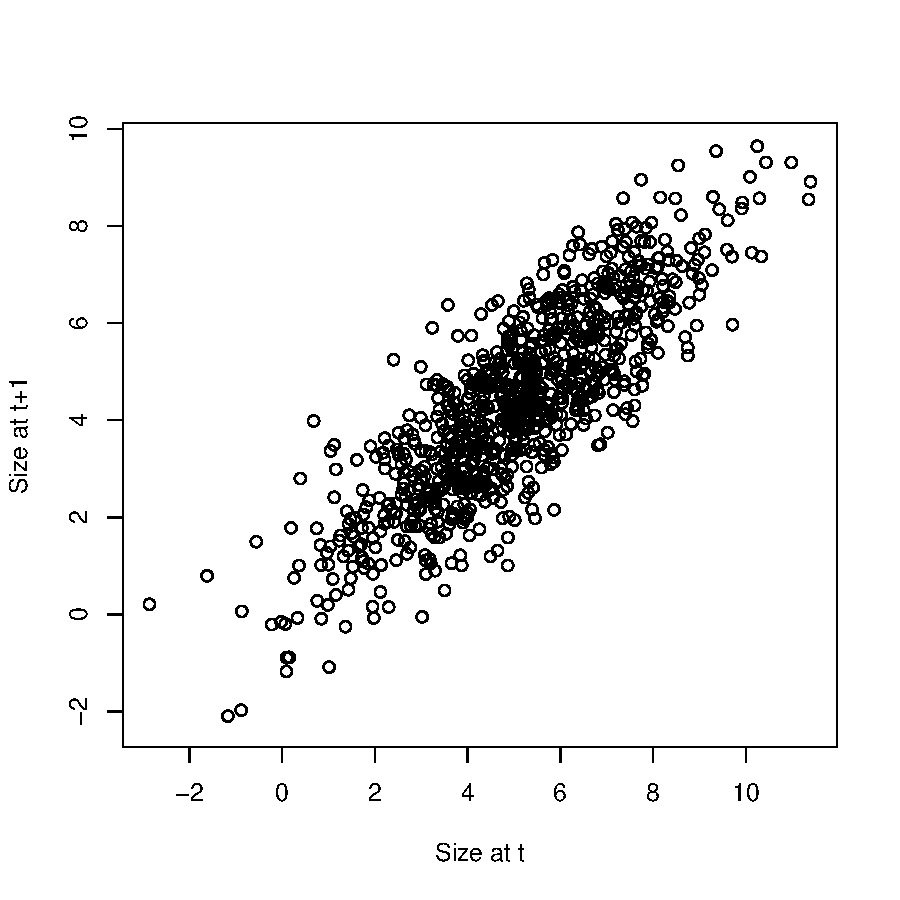
\includegraphics{IPMpack_Vignette-fig0}
\end{center}
\caption{Size at t and size at t+1}
\label{fig:zero}
\end{figure}

IPMpack is written in object-oriented code, using $S4$ objects. This means that
extra object classes are used by IPMpack, with methods assigned to those classes
that do particular things to specific objects. An example for those familiar
with $R$ is the {\tt plot} function. When applied to two vectors, it produces an x-y plot, but when applied to a fitted linear regression, it provides a series of diagnostic plots. In other words, the `plot' method is object-specific and does different things to objects of class `numeric' and objects of class `lm'.

IPMpack contains defined classes for growth, survival and fertility objects, and
associated methods that allow the user to build IPM objects. In addition, this
object-oriented structure in IPMpack uses methods from IPM objects to calculate
life expectancy, passage times, and other population estimates of interest. The
advantage of object-oriented programming is its flexibility: for example, the
same machinery can be applied to suites of underlying regression forms and the
user can take advantage of pre-existing highly generalized $R$ functions, such
as {\tt predict}. The needs of any particular dataset may require different
object and method definitions. Towards the end of this vignette we also describe how to define a new class and a new method (e.g., a new growth object for a specific life-history structure, and a new growth method applicable to plotting information from that object).

As an example, let us first define objects built as simple polynomial regressions from the generated data. The source code of {\tt generateData} will confirm that the survival data is built around a polynomial logistic regression relating size at $t$ to survival from $t$ to $t+1$, and the growth data is built around a polynomial regression relating size at $t$ to size at $t+1$. To make growth and survival objects that reflect this, the user must implement:  
\begin{Schunk}
\begin{Sinput}
> gr1 <- makeGrowthObj(dataf = dff, Formula = sizeNext~size+size2)